\documentclass[a4paper,11pt,english]{article}
\usepackage[english]{babel} 
\usepackage[T1]{fontenc}    
\usepackage[utf8]{inputenc} 
\usepackage{graphicx}       
\usepackage{hyperref}      


\begin{document}

\title{Active strategies for object discovery}
\author{Phil Bradfield \and Jan Fabian Schmid}
	
\maketitle 

\section{Introduction}
\label{Introduction}
%Introduction, which describes the motivation and goal of your project. Describe how your project is connected to existing literature. Include references to scientific papers that are relevant to your topic. Do not copy your text from the intermediate report. Revise and rewrite according to the feedback you got and what the actual outcome of the project was.

In this final report of our project, we want to present our system, how it works, how it changed during the development, and how it performs.
The goal we had for our project was to develop an autonomous robot that is able to find areas corresponding to objects in its environment.
For autonomous systems in the future it is desirable that they are able to solve everyday life tasks of humans.
Since almost every meaningful everyday life task of humans contains interaction with at least some object of the environment, it is important that robots are able to find and use objects.
One of the first steps for this is object detection, which allows the robot to filter out relevant parts of its environment which are likely to correspond to an actual object. Having a model of nearby object positions and shapes could then allow the robot to go through this internal list and search for an object that might help him for his current task.
When a robot is visiting a place for the first time it might be a good idea to explore this room to create such a list of available objects.
This is the situation and the task that we want to solve with our system.
To be able to do this, it is necessary to perform simultaneous localization and mapping, detect potential objects in the current view, and to compute the next best view (NBV) which allows to explore the environment.

\begin{figure}
	\begin{center}
		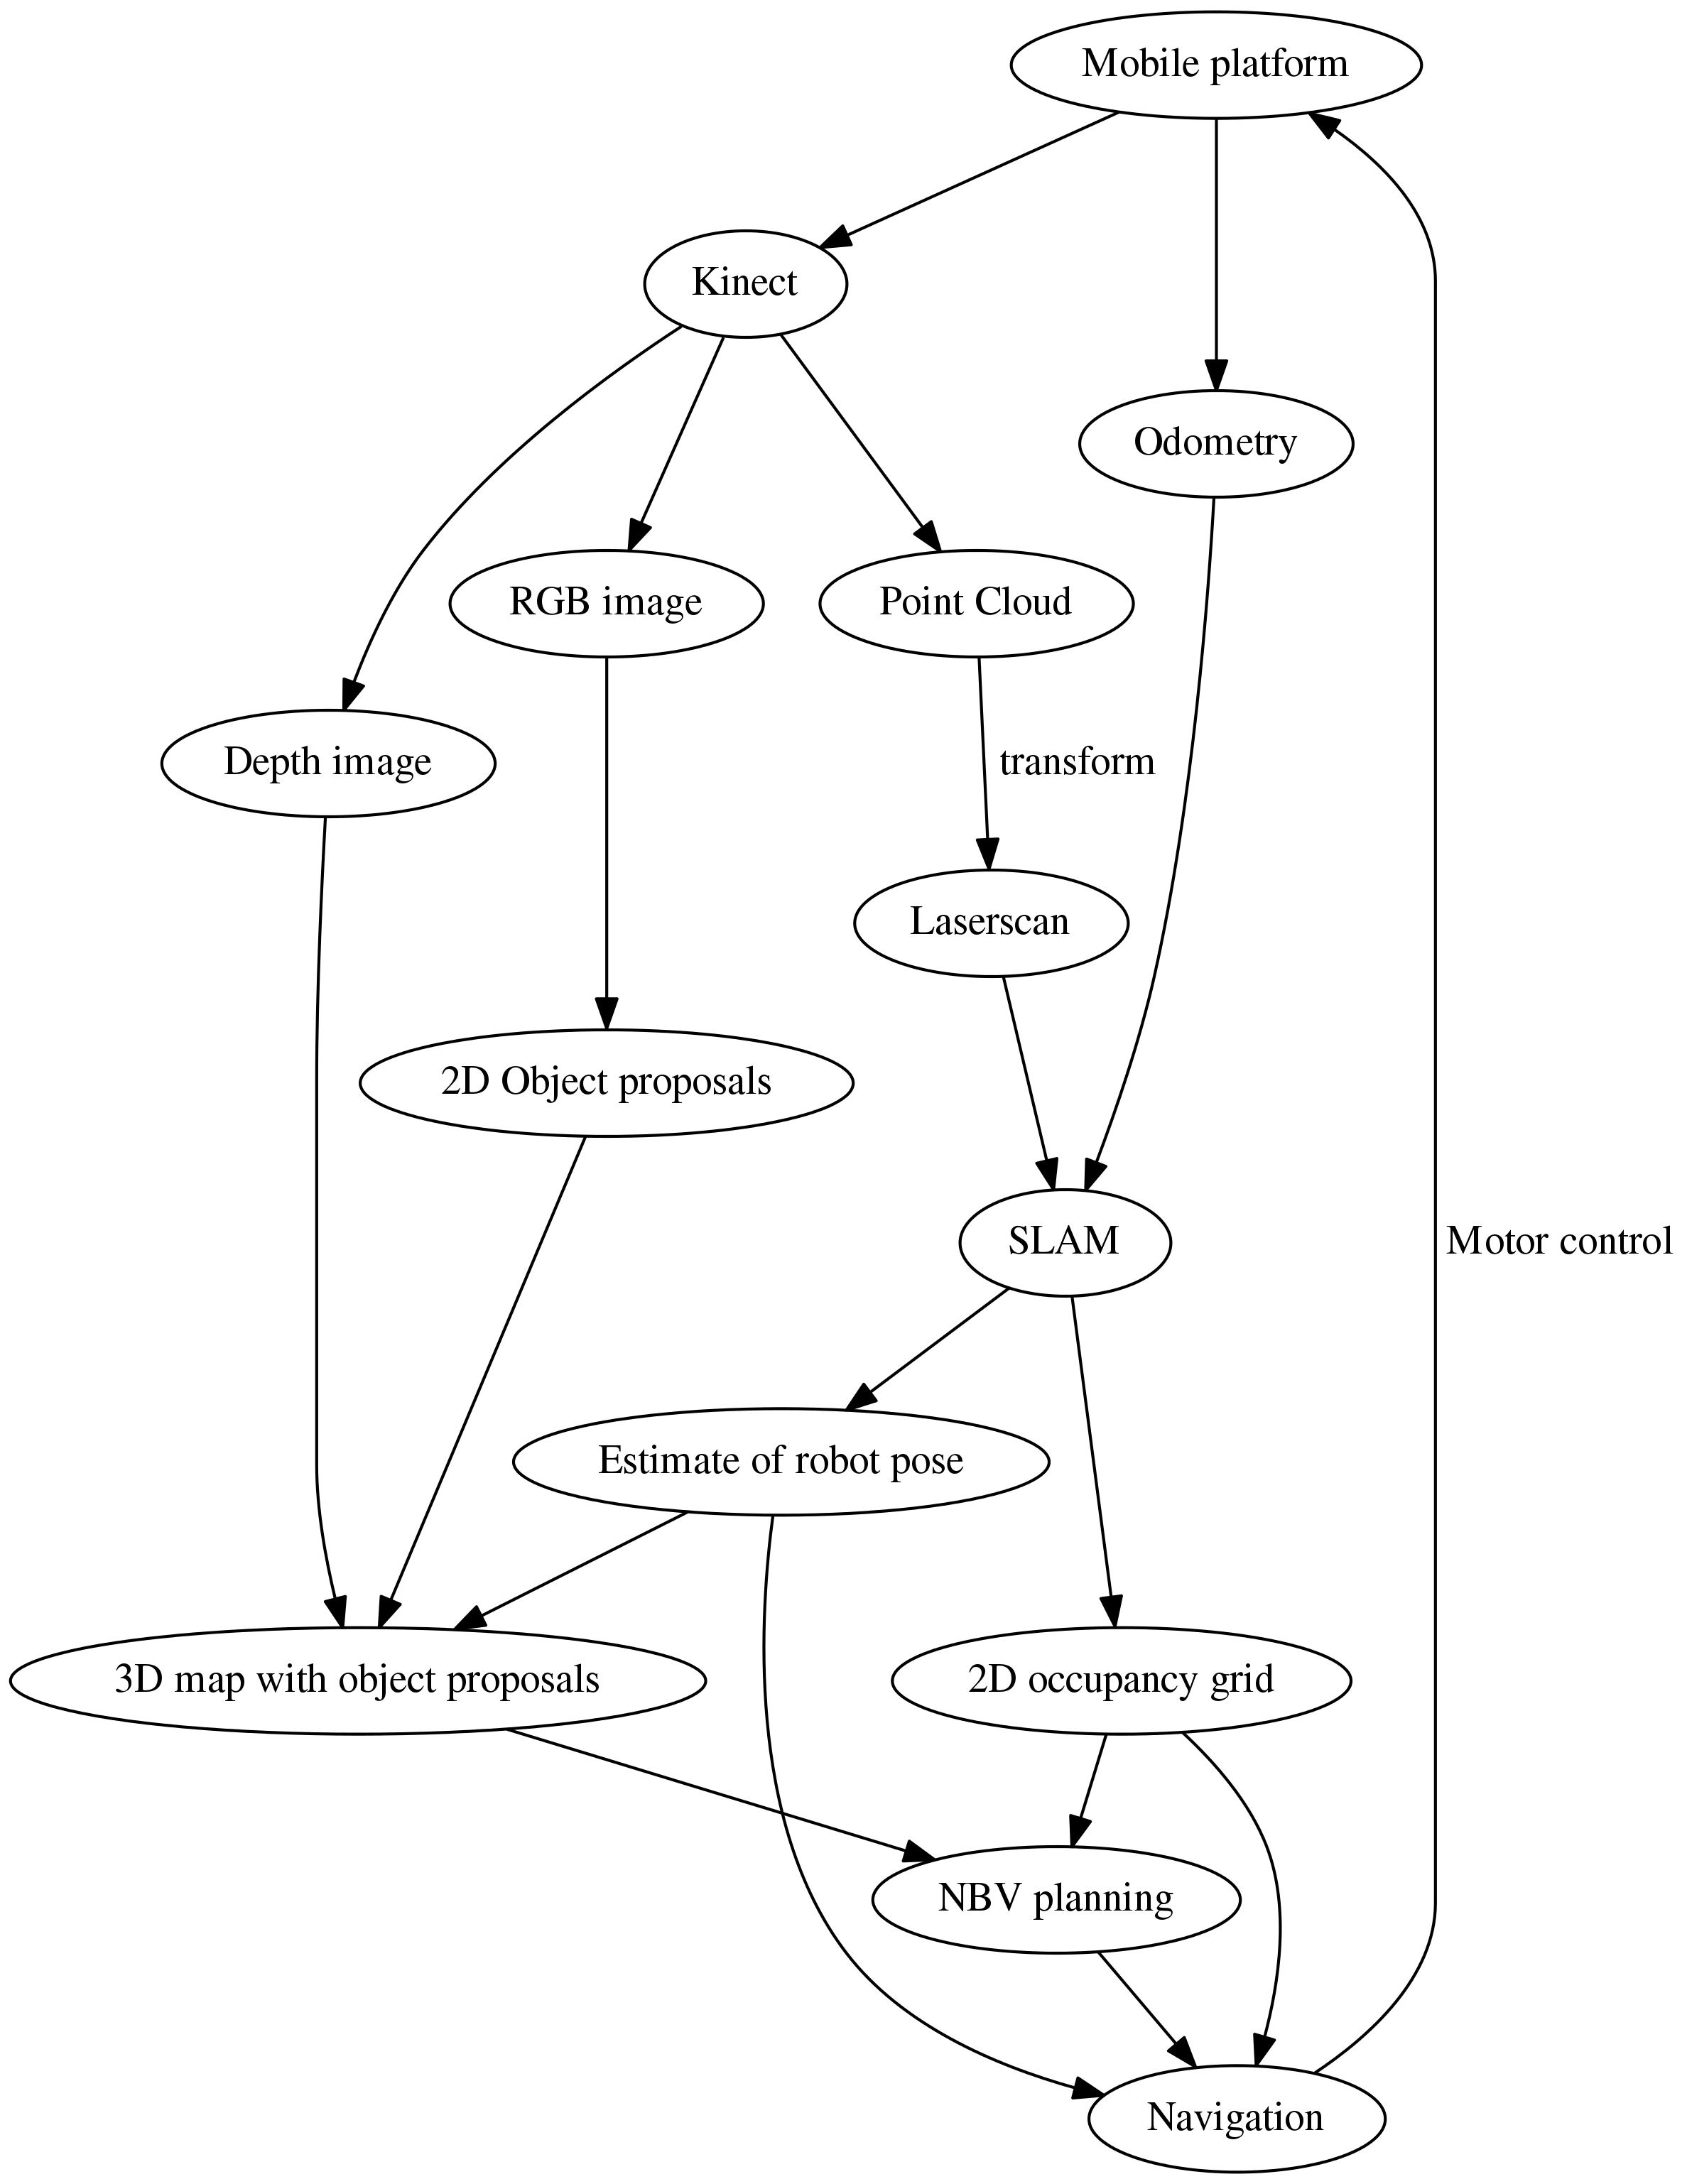
\includegraphics[width=1\linewidth]{dot/overview.png} 
		\caption{Overview of the system}
		\label{fig:overview}
	\end{center}
\end{figure}

A general overview of our system is given in Figure \ref{fig:overview}.
The available input for our computations consists of the odometry from the mobile platform and depth image, colour image, as well as point cloud data from the mounted RGB-D camera. Our SLAM algorithm requires laser scan data and the odometry, therefore we simulate a laser scanner with the point cloud data.
The SLAM algorithm provides us with an estimate of the robots current pose and a 2D occupancy grid, which is a map of the environment with information about obstacles, free space and unexplored space. 
Our object proposals are at first generated in 2D from the RGB image, then a corresponding point cloud for the object proposal is generated using the available depth information. To ensure that the object proposal point cloud corresponds to one contiguous volume a clustering algorithm is applied. Further processing is done only on the object proposal point cloud cluster closest to the robot. 
This point cloud cluster is projected, with help of the estimated robot pose, into a 3D map.
3D object proposals that already have been integrated into the map previously are updated with the new proposals.
We try different NBV algorithms, which can work with the information of the robots current pose, the 2D map of the environment, and with knowledge about the approximated object positions.
As output of each NBV algorithm we receive the next desired robot pose which is then used together with the 2D map and the approximated robot position to navigate the robot.

\medskip

A more detailed description of the implementation of the different parts of our system is given in Section \ref{Implementation}.
Previously, however, to conclude the introduction we present some existing approaches in the subject of object detection in autonomous robots and then in Section \ref{Theoretical_background} we introduce some of the core methods and concepts used for the implementation of our system.
In Section \ref{Analysis} we explain the performed experiments and obtained results of them, which allows to access the strengths and weaknesses of the system. In the end Section \ref{Conclusion} concludes this final report with a summary, a short assessment of the changes and learnings we had since the proposal of our project.

\subsection{Related work}

\section{Theoretical background}
\label{Theoretical_background}
%Theoretical background, which provides the descriptions on what existing theories and ideas that are related to your problem statement. The purpose of this section is to ensure that you are knowledgeable about the related key concepts, theories and models. Do not copy your text from the intermediate report. Revise and rewrite according to the feedback you got and what the actual outcome of the project was.

In this section we present some of the concepts and methods that we utilize in our system.

\subsection{Saliency-based object discovery}
To find objects in the robots current view, we use a saliency-based object discovery system.
Such a system has been introduced by García et al. \cite{garcia2015saliency}.
An overview of the method can be seen in Figure \ref{fig:2Dobject_discovery}.

\begin{figure}[h!]
	\begin{center}
		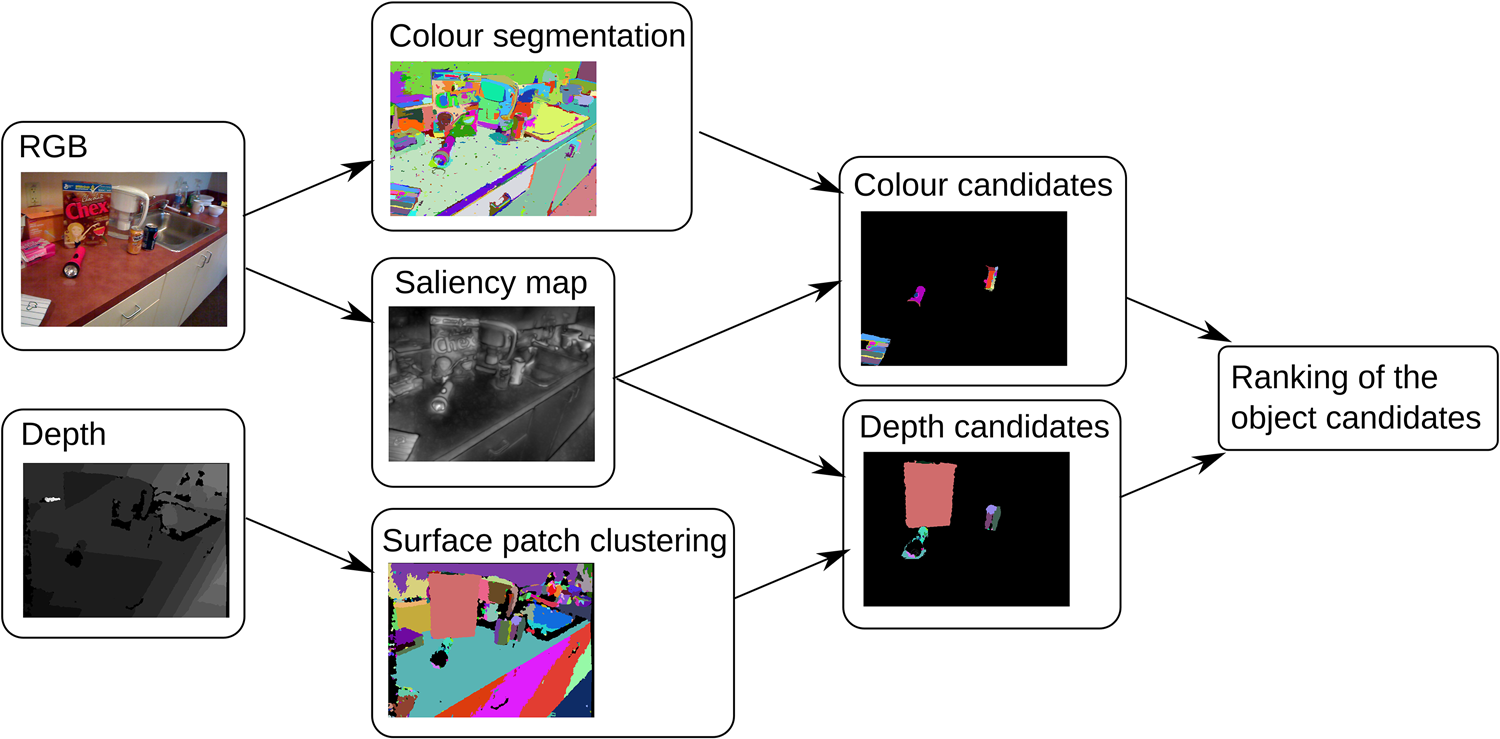
\includegraphics[width=1\textwidth]{src/saliency_object_detection.png}
		\caption{ Overview of the object candidate generation process \cite{garcia2015saliency}}
		\label{fig:2Dobject_discovery}
	\end{center}
\end{figure}

The method requires a colour and depth image of the same scene.
While it would work with colour information only experiments of the authors have shown that the combination of both achieves the best results.
The colour image is processed in two different ways: 
Using the Felzenszwalb and Huttenlocher algorithm \cite{felzenszwalb2004efficient} the image is segmented into small patches of similar colour.
Simultaneously a saliency map is computed. This is done with the VOCUS2 system developed by Frintrop et al. \cite{frintrop2015traditional}.
The general idea of VOCUS2 is to compute for each pixel a value quantifying its contrast to its proximate image area.
To generate object candidates the information of saliency map and colour segmentation are used together.
Seeded region growing is performed on the local maxima in the saliency map.
This means that starting from a local maxima neighboring pixels are iteratively grouped together into one region if their saliency value exceeds a certain percentage of the saliency value of the local maximum.
The result is a list of salient blobs in the saliency map.
For each salient blob one colour object candidate is created. It contains the pixels of all colour segments that overlap to at least $30\%$ with the pixels of the salient blob.
The depth candidates are generated analogous to the colour candidates, using the same salient blobs as a basis for the object candidates, but a surface clustering method is used as segmentation algorithm. It divides the image into continuous planes.
Afterwards, colour and depth candidates are merged into one set a ranking of proposed object candidates in terms of \glqq{}objectiveness\grqq{} takes place.

With more than 80\% recall and up to 50\% precision the saliency-based object discovery method performs comparable or better than other state-of-the-art object detection systems tested in the experiments of García et al.

\subsection{Frontier-based exploration}
A method for autonomous exploration of unknown  environments has been introduced 1997 by Yamauchi \cite{yamauchi1997frontier}.
He describes the task that he wants to solve as follows: \glqq{}The central question in exploration is: \textit{Given what you know about the world, where should you move to gain as much  new  information  as  possible?}\grqq{}.
This is the same problem we have to solve for our object seeking robot.
Figure \ref{fig:frontier} presents how frontier-based exploration works.

\begin{figure}[h!]
	\begin{center}
		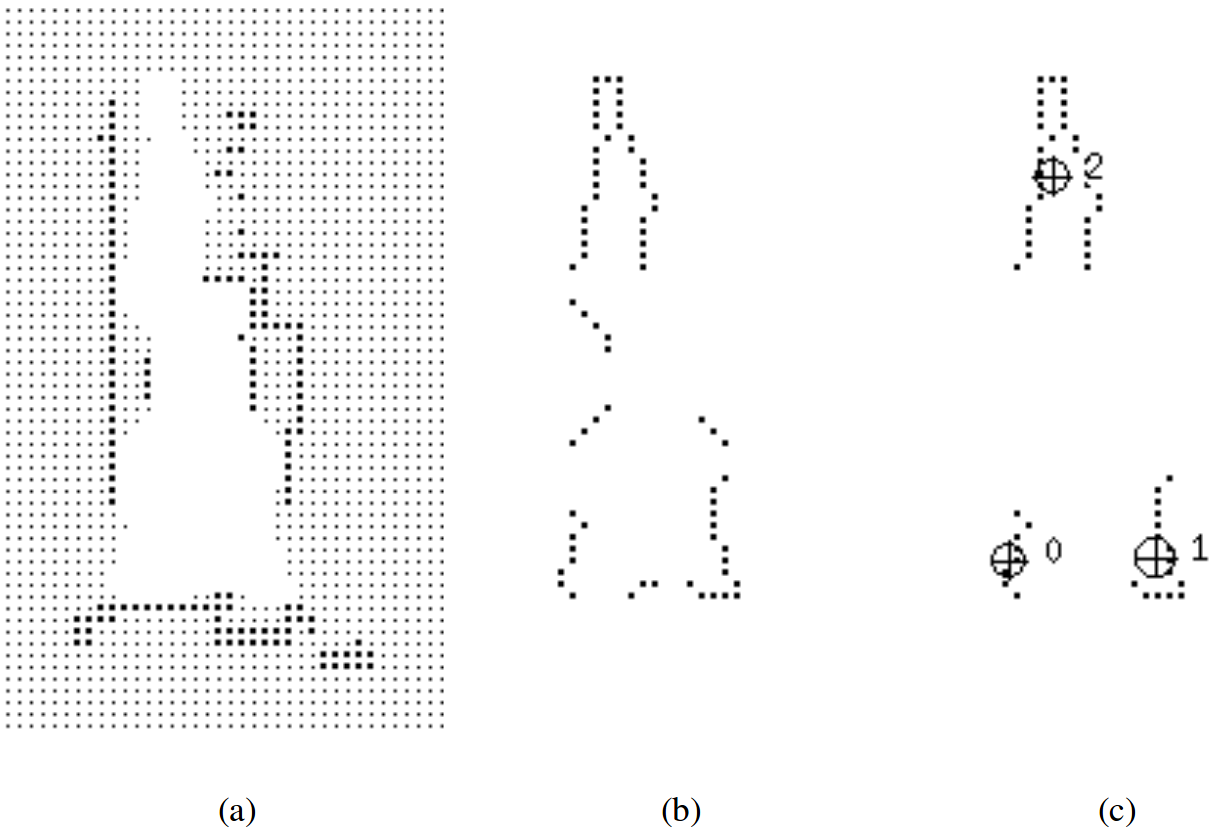
\includegraphics[width=1\textwidth]{src/frontier_exploration.png}
		\caption{ Processing steps of frontier-based exploration \cite{yamauchi1997frontier}}
		\label{fig:frontier}
	\end{center}
\end{figure}

On the left (a) of the figure a possible map of the environment is depicted. Black dots represent unexplored cells of the map, stronger black dots mark found obstacles and white space is the available free space in which the robot should be able to navigate.
All cells on the border between free and unexplored space are marked in (b) as frontier edge segments.
Neighboring frontier edge segments are grouped together and if the contiguous space of the group is roughly larger than the robot, the group defines a frontier. The centroid of each frontier is represented by a crosshair in (c).
The robot will then navigate to the closest accessible frontier centroid and thereby explore the environment.

Yamauchi performed successful experiments using a Nomad 200 mobile robot in indoor environments.

\subsection{Sampling-based exploration}
Sampling-based exploration is another way of finding a next best viewpoint to explore an initially unknown environment.
The general idea is to randomly sample the accessible area of the robot for possible viewpoints.
For each viewpoint a information gain score is computed, which depends on the visible area at the particular viewpoint and the distance of this viewpoint to the current robot position.

Such a system has been introduced by Surmann et al. \cite{surmann2003autonomous}.
For their system they use laser scanner data. From this data they detect obstacles, free space and unknown space.
The borders between free space and unknown space are called unseen lines.
Next best viewpoint candidates are randomly sampled from the free space.
For each of these candidates the number of visible unseen lines is computed, which determines its information gain.
The final score for each candidate is computed by multiplying the information gain with a punishing factor that depends on the euclidean distance to the current robot position and the angle that the robot would have to rotate for the view.
The next goal is then chosen as the viewpoint candidate with highest overall score.

%\subsection{Particle filter SLAM}
%\subsection{Euclidean point cloud clustering}
\subsection{IoR mechanism to guide attention}
An inhibition of return (IoR) mechanism can be used in computer vision to avoid spending attention on the same region for longer than necessary to process the information of that region.
Such a method is used in the object detection system by García et al. \cite{garcia2015saliency} to avoid the computation of the same object candidates in consecutive frames of a video sequence.
The system keeps track of previously considered object candidates through an 3D IoR map, which is a model of the environment built through a reconstruction algorithm (KinectFusion \cite{newcombe2011kinectfusion}) from the depth image of the RGB-D camera, where information about IoR is stored in the voxels of the map.
To update the IoR information in the map the current 2D camera frame is projected into the 3D map.
That way, voxels corresponding to the attended object candidates are found.
The IoR weight for each of these voxels is increased and if a certain threshold is reached an IoR flag is activated, signaling that pixels in the camera frame corresponding to this voxel should be inhibited.
For each frame that a voxel is not attended its IoR weight decreases and if it reaches zero again the IoR flag is deactivated.

The integration of this 3D IoR mechanism allowed García et al. to find most of the visible objects in a video while considering only a few object candidates per frame.

\subsection{Building a 3D map with octomap data structure}

\section{Implementation}
\label{Implementation}
%Implementation, which connects with the section on theoretical background and describes how the required parts were implemented, and how the overall system is constructed.

The general structure of our system has been introduced in Section \ref{Introduction} already.
We have mostly developed our system inside a physics simulation (Gazebo \footnote{\url{http://gazebosim.org/}}), however we transferred the system with slight adjustments onto a real Pioneer robot as well.
In the following we will explain how the different parts in Figure \ref{fig:overview} have been implemented. If the simulated and real version are diverging we will point that out in the respective system part description.
The system is fully developed with the Robot Operating System (ROS \footnote{\url{http://www.ros.org/}}) in the Indigo version, therefore each part of the system consists of one or multiple ROS nodes and services.
The code for our system can be found online \footnote{\url{https://github.com/Fabse92/cv_project}}.

\subsection{Mobile platform}
As mobile platform we used a Pioneer P3DX. This robot is providing a first estimate for its own position in form of odometry based on the previous motor control. Mounted onto the platform is a Kinect camera \footnote{\url{https://developer.microsoft.com/en-us/windows/kinect}}. In case of the real version we put the camera on top of the platform, in the physics simulation we are free of physical bounds and put the camera slightly lower in front of the robot to accommodate for our experimental setup in which objects are lying scattered on the floor.

\subsection{RGB-D camera}
The Kinect camera is directly providing a rectified version of the colour and depth image, which aligns the two frames, therefore pixel coordinates both images are corresponding to each other (\textbf{TODO is this correct?!}).
Also a point cloud build from the fused information of depth and colour image is directly provided as a ROS topic through the respective camera driver for simulation and real world.

\subsection{Laserscan}
To simulate a laser scanner we use the ros package \textit{pointcloud\_to\_laserscan} \footnote{\url{http://wiki.ros.org/pointcloud_to_laserscan}}.
It receives the current point cloud from the RGB-D camera and samples the point cloud between a specified minimal and maximal height.
The closest point for each vertical line is put out to form one horizontal line which is our simulated laser scan.

\subsection{SLAM}
To solve the simultaneous localization and mapping problem we used the ROS package \textit{GMapping} \footnote{\url{http://wiki.ros.org/gmapping}}.
GMapping performs laser-based SLAM using a particle filter.
It requires laser scan data and the estimated current robot position and provides a 2D occupancy grid map and the transform of the robot's pose into the map frame.
The occupancy grid map consists of cells of specified size.
Each cell can take one of four possible values.
The cell is thereby marked as obstacle, free space, unexplored space or as inscribed inflated obstacle, which means that this cell is not accessible by the robot since according to its footprint it would be in collision with an obstacle.

\subsection{Generation of object proposals}
The generation of object proposals is a complex part of the system that consists of five separate processing steps that we describe individually.

\subsubsection{2D Object candidate generation}
\subsubsection{Building the proposal point cloud}
\subsubsection{Clustering the point cloud}
\subsubsection{Projection of point cloud into map}
\subsubsection{Merging and handling of candidates in octomap}

\subsection{NBV planning}
In our current system five different next best view algorithms are available, which we will describe in their individual parts.
The goal of each of these algorithms is to find a next view point with high information gain.

\subsubsection{Random NBV}
\subsubsection{Frontier exploration}
\subsubsection{Sampling-based exploration using obstacles}
IoR mechanism for obstacles
\subsubsection{Sampling-based exploration using obstacles and object proposals}
\subsubsection{Combination of Frontier and Sampling based exploration}

\subsection{Navigation}
For navigation we use the \textit{move\_base} ROS package \footnote{\url{http://wiki.ros.org/move_base}}.
It requires the current robot position approximation, sensor transforms and sensor data and provides appropriate velocity commands to navigate the platform once a valid goal pose has been made public.

\section{Analysis}
\label{Analysis}
% Results, which contain the descriptions of the experiments conducted and presents their results.

\subsection{Experimental setups}
\subsection{Metrics}
\subsection{Results}

\section{Conclusion}
\label{Conclusion}
%Conclusions, which summarizes the work that was done and the results obtained, and gives suggestions for future work. \textbf{Most importantly}, include a section that contrasts the actual outcome of the project to the plan you submitted: what was planned, what was actually achieved, what were the main reasons for the actual outcome, what you consider you have learned during the project, etc.

\subsection{Summary}
\subsection{Learnings and deviations from our original plans}
\subsection{Future work}

\newpage
\bibliographystyle{plain}
\addcontentsline{toc}{section}{Bibliography}% Add to the TOC
\bibliography{bib}

\end{document}
